\chapter{Metodología y herramientas}
\label{chap:metodologia}

\drop{E}{ste} capítulo presenta el marco metodológico completo que ha guiado
el desarrollo de \dataqual.  Se expone, en primer lugar, la metodología ágil
de gestión del proyecto (Scrum adaptado a un entorno individual), junto con
su justificación y adaptación práctica.  A continuación se describe la
metodología de desarrollo de software adoptada, el stack tecnológico
seleccionado y el entorno de trabajo.  El capítulo concluye con la
planificación temporal del proyecto mediante un diagrama de Gantt, la
estimación del esfuerzo, el análisis de costes y el plan de gestión de
riesgos.


%% =========================================================================
\section{Gestión del proyecto}
\label{sec:gestion-proyecto}
%% =========================================================================

\subsection{Metodología ágil adoptada: Scrum adaptado}

Para la gestión del proyecto se adoptó \textbf{Scrum adaptado a un proyecto
unipersonal}~\citep{scrumguide}, una metodología ágil que organiza el trabajo
en sprints de duración acotada y favorece la entrega incremental de valor.
La elección se justifica por tres razones:

\begin{itemize}
  \item \textbf{Adecuación al tipo de proyecto.}  Los requisitos de \dataqual
    no estaban completamente definidos desde el inicio: a medida que se
    profundizaba en el dominio de la calidad de datos y los estándares ISO,
    surgían nuevas necesidades que había que incorporar al backlog.  Scrum
    encaja bien con este tipo de proyectos exploratorios e iterativos.

  \item \textbf{Retroalimentación continua.}  La estructura de sprints
    facilita la revisión periódica del incremento con los tutores,
    permitiendo ajustar prioridades y corregir la dirección del proyecto
    antes de que las desviaciones sean costosas.

  \item \textbf{Trazabilidad del avance.}  Cada sprint produce un conjunto
    delimitado de entregables, lo que genera un histórico auditable del
    progreso y facilita la redacción de las retrospectivas incluidas en
    el Capítulo~\ref{chap:desarrollo}.
\end{itemize}

La adaptación concreta de Scrum a este proyecto se detalla en la
subsección siguiente.

\subsection{Adaptación de Scrum al TFG individual}

Dado que Scrum está concebido para equipos de entre tres y nueve personas,
su aplicación a un proyecto unipersonal requiere simplificar los roles y
adaptar los eventos sin perder el núcleo del marco: sprints de duración
acotada, backlog priorizado e inspección y adaptación continuas.  Las
adaptaciones adoptadas se detallan a continuación.

\begin{definitionlist}
  \item[Sprints]  El proyecto se divide en \textbf{6 sprints} de duración
    variable entre cuatro y ocho semanas, ajustada a la complejidad de cada
    incremento.  La duración variable es una adaptación deliberada: los
    sprints de mayor carga técnica (S2, S6) reciben más tiempo, mientras
    que los de alcance más acotado (S3--S5) se mantienen en un mes.
    La distribución temporal completa se recoge en la
    Sección~\ref{sec:planificacion}.

  \item[Roles]  Al ser un proyecto individual, el estudiante asume
    simultáneamente los tres roles de Scrum:
    \begin{itemize}
      \item \emph{Product Owner}: define y prioriza el backlog en función de
        los objetivos del \ac{TFG} y de la retroalimentación de los tutores.
      \item \emph{Scrum Master}: vela por la aplicación coherente de la
        metodología y gestiona los bloqueos técnicos o de planificación.
      \item \emph{Developer}: implementa las historias de usuario
        seleccionadas para cada sprint.
    \end{itemize}

  \item[Sprint planning]  Al inicio de cada sprint se define el objetivo,
    se seleccionan las historias de usuario del backlog y se descomponen en
    tareas concretas registradas en Trello con estimación en horas.

  \item[Daily standup]  Sustituido por una \textbf{revisión personal diaria}
    informal: al comenzar cada sesión de trabajo se repasaba el estado de
    las tareas en curso y se decidía el foco de la jornada.

  \item[Sprint review]  Al finalizar cada sprint (o cada dos en los meses de
    mayor densidad de trabajo) se acordaba una reunión con los tutores para
    revisar el incremento funcional y ajustar las prioridades del backlog.
    La convocatoria era bajo demanda, sin cadencia fija, para adaptarla al
    ritmo real del proyecto.

  \item[Sprint retrospective]  Reflexión escrita al cierre de cada sprint
    siguiendo un guión estructurado: logros del sprint, estado acumulado del
    producto, incidencias detectadas, estimación frente a tiempo real y
    acción de mejora para el sprint siguiente.  Las retrospectivas completas
    se recogen en el Capítulo~\ref{chap:desarrollo}.
\end{definitionlist}

Esta adaptación conserva los elementos esenciales de Scrum (iteraciones
cortas, entregables funcionales y mejora continua) mientras prescinde de
los eventos que carecen de sentido en un contexto unipersonal, como el
\emph{daily standup} en grupo o la \emph{sprint review} formal ante el
equipo.

\subsection{Herramientas de gestión}

La gestión del proyecto se apoyó en dos herramientas complementarias:
Trello para el seguimiento ágil del backlog y Git + GitHub para el
control de versiones del código fuente.

\begin{definitionlist}
  \item[Trello]  Herramienta principal de gestión del backlog y
    seguimiento de sprints.  Cada historia de usuario y tarea técnica
    se representa como una tarjeta con prioridad, estimación en horas
    y estado.  El tablero Kanban organiza las tarjetas en cinco
    columnas (\textit{Backlog}, \textit{Sprint actual},
    \textit{En progreso}, \textit{En revisión / Iterable},
    \textit{Terminado}), lo que permite visualizar
    el flujo de trabajo tanto dentro de cada sprint como la progresión
    entre sprints.

  \item[Git + GitHub]  Sistema de control de versiones distribuido con
    repositorio remoto en GitHub.  El desarrollo se realizó
    principalmente sobre la rama \texttt{main}, creando ramas de
    funcionalidad (\emph{feature branches}) únicamente para las tareas
    de mayor envergadura o riesgo.  Los mensajes de \emph{commit}
    siguen una convención descriptiva que facilita la trazabilidad de
    los cambios y la redacción de las retrospectivas.
\end{definitionlist}

Ambas herramientas son de acceso libre y gratuito, lo que se refleja
en la estimación de costes de la Sección~\ref{sec:costes}.


%% =========================================================================
\section{Metodología de desarrollo}
\label{sec:metodologia-desarrollo}
%% =========================================================================

El desarrollo de \dataqual ha seguido una \textbf{metodología iterativa e
incremental}, donde cada sprint produce un incremento funcional desplegable
que amplía las capacidades de la plataforma.  Los principios que han guiado
todo el proceso (entrega frecuente, retroalimentación continua y adaptación
del plan ante nuevos requisitos) son coherentes con los valores del
\emph{Agile Manifesto}~\citep{agilemanifesto}.

\subsection{Desarrollo iterativo}

El proyecto se ha organizado en \textbf{iteraciones} de duración variable
(entre cuatro y ocho semanas), cada una de las cuales ha producido un
incremento funcional desplegable.  Cada iteración ha comprendido las
siguientes actividades:

\begin{enumerate}
  \item \textbf{Planificación:} selección de las funcionalidades a
    implementar en la iteración, priorizando aquellas que aportan mayor valor
    o que desbloquean funcionalidades posteriores.

  \item \textbf{Diseño:} definición de la arquitectura y el modelo de datos
    necesarios para las funcionalidades seleccionadas, tomando como referencia
    los estándares \ac{ISO}/IEC~25012~\citep{iso25012} e
    \ac{ISO}/IEC~5259~\citep{iso5259} para el diseño de las métricas de
    calidad.

  \item \textbf{Implementación:} desarrollo del código del \emph{backend} y
    del \emph{frontend} de forma conjunta, garantizando que cada incremento
    sea funcional de extremo a extremo.

  \item \textbf{Verificación:} ejecución de pruebas manuales y automatizadas
    para validar el correcto funcionamiento del incremento.

  \item \textbf{Revisión con los tutores:} presentación del avance para
    obtener retroalimentación y ajustar la dirección del desarrollo en caso
    necesario.
\end{enumerate}

Este ciclo se repite en cada sprint y puede observarse con detalle en las
secciones de planificación y retrospectiva del
Capítulo~\ref{chap:desarrollo}.

\subsection{Prototipado}

La interfaz de usuario se ha desarrollado siguiendo un enfoque de
\textbf{prototipado evolutivo}: cada pantalla se construyó inicialmente
con la funcionalidad mínima necesaria y se refinó en iteraciones sucesivas,
incorporando mejoras de usabilidad, visualizaciones adicionales y tratamiento
de casos extremos.  Este enfoque permitió validar la experiencia de usuario
de forma temprana sin invertir tiempo excesivo en el diseño visual antes de
confirmar la utilidad funcional.

Un ejemplo representativo es el módulo de exploración de datos (\ac{EDA}):
en su primera versión solo mostraba un recuento de nulos y estadísticas
básicas por columna; en iteraciones posteriores se incorporaron histogramas
interactivos, diagramas de caja y una matriz de correlación, a medida que
las pruebas con datos reales revelaban la necesidad de cada visualización.


%% =========================================================================
\section{Pila tecnológica}
\label{sec:pila-tecnologica}
%% =========================================================================

La pila tecnológica de \dataqual se estructura en cuatro capas
independientes pero integradas: presentación (\emph{frontend}), lógica de
negocio (\emph{backend}), persistencia de datos y orquestación asíncrona.
La selección de cada tecnología responde a tres criterios: adecuación al
tipo de problema (evaluación de calidad de datos, procesamiento asíncrono,
visualización interactiva), madurez y soporte comunitario, y coherencia con
las competencias adquiridas durante el grado en Ingeniería Informática.

\subsection{\emph{Frontend}}
\label{sec:tech-frontend}

La capa de presentación se construyó sobre Next.js y React, combinación que
ofrece enrutamiento basado en ficheros, reescritura de rutas para actuar
como \emph{proxy} hacia el \emph{backend} y generación de contenido
estático.  Se descartó Vue.js por su ecosistema de componentes de
visualización menos maduro en el momento del desarrollo.  TypeScript se
incorporó desde el inicio para garantizar la seguridad de tipos en un
\emph{frontend} con más de cuarenta componentes reutilizables.
La Tabla~\ref{tab:tech-frontend} recoge el detalle de cada tecnología.


\begin{table}[htbp]
  \centering
  \caption{Tecnologías del \emph{frontend}}
  \label{tab:tech-frontend}
  \begin{tabularx}{\textwidth}{l l X}
    \toprule
    \textbf{Tecnología} & \textbf{Versión} & \textbf{Justificación} \\
    \midrule
    Next.js   & 13.3 & \emph{Framework} React con enrutamiento basado en
      ficheros, reescritura de rutas para \emph{proxy} al \emph{backend} y
      modo \emph{standalone} para Docker. \\
    React     & 18   & Biblioteca estándar para interfaces de usuario.  Los
      \emph{hooks} y la Context \ac{API} eliminan la necesidad de gestores de
      estado externos como Redux. \\
    TypeScript & 5.0 & Tipado estático que detecta errores en tiempo de
      compilación, esencial para mantener un \emph{frontend} con más de
      cuarenta componentes. \\
    Material \ac{UI} & 5.12 & Biblioteca de componentes con \emph{theming},
      diseño adaptable y accesibilidad incorporada. \\
    Chart.js  & 4.2  & Biblioteca de gráficos ligera con soporte para
      histogramas, diagramas de dispersión y de líneas.  Se utiliza mediante
      el \emph{wrapper} \texttt{react-chartjs-2}. \\
    Axios     & 1.3  & Cliente HTTP con interceptores para inyección
      automática de \ac{JWT} y gestión centralizada de errores. \\
    \bottomrule
  \end{tabularx}
\end{table}

\subsection{\emph{Backend}}
\label{sec:tech-backend}

El \emph{backend} se implementó en Python con Flask como \emph{framework}
web.  Python fue la elección natural por su integración nativa con las
bibliotecas de análisis de datos (Pandas, NumPy) que sustentan el motor de
métricas.  Flask se prefirió frente a Django porque no impone una estructura
monolítica, lo que permitió diseñar una arquitectura modular basada en
\emph{blueprints} a medida de los requisitos del sistema; además, el
autor contaba con experiencia previa con este \emph{framework}, lo que
redujo la curva de aprendizaje y aceleró el desarrollo inicial.
La Tabla~\ref{tab:tech-backend} recoge el detalle de cada biblioteca y
herramienta empleada.


\begin{table}[htbp]
  \centering
  \caption{Tecnologías del \emph{backend}}
  \label{tab:tech-backend}
  \begin{tabularx}{\textwidth}{l l X}
    \toprule
    \textbf{Tecnología} & \textbf{Versión} & \textbf{Justificación} \\
    \midrule
    Python    & 3.10 & Lenguaje estándar en ciencia de datos e \ac{IA}, con
      excelente integración con Pandas y NumPy para el cálculo de
      métricas. \\
    NumPy     & 1.24 & Cálculo numérico de alto rendimiento sobre arrays.
      Se emplea en el motor de métricas para operaciones vectorizadas sobre
      columnas del conjunto de datos. \\
    Flask     & 2.2  & \emph{Framework} web minimalista y flexible, ideal
      para \ac{API}s \ac{REST}.  No impone una estructura fija, lo que
      permite una arquitectura a medida. \\
    SQLAlchemy & 2.0 & \ac{ORM} maduro con soporte completo para PostgreSQL,
      incluyendo campos JSONB, tipos \texttt{ENUM} y \emph{pool} de
      conexiones integrado. \\
    Flask-JWT-Extended & 4.4 & Autenticación \ac{JWT} con \emph{tokens} de
      acceso y refresco, \emph{blacklisting} y gestión de errores
      personalizada. \\
    Flask-Migrate & 4.0 & Migraciones de base de datos versionadas con
      Alembic, que permiten evolucionar el esquema de forma controlada. \\
    Pandas    & 1.5  & Manipulación de datos tabulares: lectura de conjuntos
      de datos, cálculo de métricas y generación de estadísticas
      descriptivas. \\
    Gunicorn  & 20.1 & Servidor \ac{WSGI} de producción con soporte
      multiproceso para gestionar la concurrencia. \\
    \bottomrule
  \end{tabularx}
\end{table}

\subsection{Base de datos y almacenamiento}
\label{sec:tech-bbdd}

La capa de persistencia separa deliberadamente dos tipos de datos con
naturaleza distinta: los datos relacionales (proyectos, usuarios, métricas,
resultados) se almacenan en PostgreSQL, mientras que los ficheros binarios
subidos por los usuarios se delegan a MinIO.  Esta separación evita saturar
la base de datos relacional con objetos de gran tamaño y simplifica el
escalado independiente de cada almacén.  Redis actúa además como
intermediario de mensajes para el sistema de colas asíncronas.
La Tabla~\ref{tab:tech-bbdd} detalla cada componente de esta capa.


\begin{table}[htbp]
  \centering
  \caption{Tecnologías de base de datos y almacenamiento}
  \label{tab:tech-bbdd}
  \begin{tabularx}{\textwidth}{l l X}
    \toprule
    \textbf{Tecnología} & \textbf{Versión} & \textbf{Justificación} \\
    \midrule
    PostgreSQL & 14  & Sistema de gestión de bases de datos relacional con
      soporte nativo para JSONB, tipos \texttt{ENUM} e índices avanzados.
      Permite combinar datos estructurados (relaciones entre entidades) con
      datos semiestructurados (configuraciones, resultados). \\
    MinIO     & \emph{latest} & Almacenamiento de objetos compatible con S3,
      autoalojado.  Separa los archivos binarios de los datos relacionales y
      mantiene los datos en la infraestructura propia sin depender de
      servicios externos en la nube. \\
    Redis     & 6    & Almacén en memoria con rol dual: \emph{broker} de
      mensajes para Celery y \emph{storage} para el limitador de tasa de
      peticiones.  Su baja latencia es idónea para la gestión de colas. \\
    \bottomrule
  \end{tabularx}
\end{table}

\subsection{Procesamiento asíncrono y orquestación}
\label{sec:tech-async}

La ejecución de evaluaciones de calidad puede tardar varios segundos en
conjuntos de datos de tamaño medio, por lo que realizarla de forma síncrona
bloquearía la interfaz de usuario.  Celery resuelve este problema
desacoplando la petición del usuario de la ejecución real de la tarea: el
\emph{frontend} lanza la evaluación, recibe un identificador de tarea y
consulta el estado periódicamente hasta que finaliza.  Docker y Docker
Compose unifican todos los servicios en un entorno reproducible que se
despliega con un único comando.
La Tabla~\ref{tab:tech-async} detalla las herramientas que componen esta
capa.


\begin{table}[htbp]
  \centering
  \caption{Tecnologías de procesamiento asíncrono y orquestación}
  \label{tab:tech-async}
  \begin{tabularx}{\textwidth}{l l X}
    \toprule
    \textbf{Tecnología} & \textbf{Versión} & \textbf{Justificación} \\
    \midrule
    Celery    & 5.2  & Cola de tareas distribuida estándar en Python, con
      soporte para reintentos, \emph{timeouts} y seguimiento de progreso.
      Escalable horizontalmente mediante la adición de
      \emph{workers}~\citep{celery}. \\
    Flower    & 1.2  & Cuadro de mando web para la monitorización en tiempo
      real de \emph{workers}, tareas y colas de Celery. \\
    Docker    & ---  & Contenedorización de cada servicio, garantizando
      aislamiento de dependencias, portabilidad y
      reproducibilidad~\citep{docker}. \\
    Docker Compose & --- & Orquestación de los ocho servicios con
      \emph{healthchecks}, volúmenes persistentes, red interna y variables de
      entorno.  Un único comando (\texttt{docker-compose~up}) despliega el
      \emph{stack} completo. \\
    \bottomrule
  \end{tabularx}
\end{table}

El conjunto de estas cuatro capas forma una arquitectura desacoplada en la
que cada componente puede sustituirse o escalarse de forma independiente.
Todas las tecnologías seleccionadas son de código abierto, lo que elimina
costes de licencia y garantiza la reproducibilidad del entorno de desarrollo
y despliegue.


%% =========================================================================
\section{Entorno de desarrollo}
\label{sec:entorno-desarrollo}
%% =========================================================================

El entorno de desarrollo está íntegramente basado en herramientas de
código abierto y gratuitas, lo que garantiza que cualquier colaborador
pueda reproducir el entorno sin coste adicional.

\begin{definitionlist}
  \item[Editor de código]  Visual Studio Code, con extensiones para
    Python (Pylance), TypeScript, Docker y \LaTeX{} (LaTeX Workshop).

  \item[Entorno de ejecución local]  Docker Desktop sobre Windows~11,
    con Docker Compose para levantar los ocho servicios de forma
    simultánea.  Este enfoque elimina la necesidad de instalar
    dependencias directamente en el sistema operativo anfitrión.

  \item[Gestor de paquetes \emph{frontend}]  pnpm, seleccionado por su
    eficiencia en el uso de disco y su velocidad de instalación frente
    a npm.

  \item[Gestor de paquetes \emph{backend}]  pip con fichero
    \texttt{requirements.txt} para la gestión de dependencias Python.

  \item[Pruebas]  pytest como \emph{framework} de pruebas del
    \emph{backend}, con soporte para pruebas unitarias y de integración.
\end{definitionlist}

El conjunto de estas herramientas, combinado con la contenedorización de
todos los servicios, permite que el entorno de desarrollo sea
indistinguible del entorno de producción, reduciendo los problemas
habituales de incompatibilidad entre plataformas.


%% =========================================================================
\section{Planificación temporal}
\label{sec:planificacion}
%% =========================================================================

El desarrollo del proyecto se ha distribuido a lo largo del curso académico
2025--2026 en seis fases encadenadas.  Las dos primeras sentaron las bases del
sistema: entre octubre y noviembre~2025 se estudió el estado del arte y se
analizaron los estándares \ac{ISO}/IEC~25012~\citep{iso25012} e
\ac{ISO}/IEC~5259~\citep{iso5259}, lo que permitió diseñar la arquitectura
general; durante diciembre~2025 y enero~2026 se implementó el núcleo del
\emph{backend}: modelos de datos, autenticación \ac{JWT}, módulo de ingesta
multiformato con almacenamiento en MinIO y esqueleto de la \ac{API}
\ac{REST}ful.

Las fases centrales construyeron el núcleo funcional. En febrero~2026 se
diseñó e implementó el motor de métricas con arquitectura de \emph{plugins}
(clase base abstracta y registro dinámico) y las tres primeras métricas de
calidad.  En marzo~2026 se concentró el desarrollo del \emph{frontend} con
Next.js y React: cuadros de mando, páginas de gestión y el módulo de
exploración de datos (\ac{EDA}), si bien desde las fases anteriores ya
existía una interfaz básica operativa; paralelamente se incorporaron nuevas
métricas al catálogo.

Las dos últimas fases elevaron la madurez del sistema y cerraron el proyecto.
Abril~2026 se dedicó a las funcionalidades avanzadas: \emph{fingerprinting} de
\emph{issues}, \emph{Quality Gates}, comparación con línea base y
enmascaramiento de \ac{PII}; en este mismo sprint se completó el catálogo de
métricas con las restantes, incluida la métrica de diversidad.  La fase final
(mayo--junio~2026) abarca la redacción de la memoria, la validación con datos
reales y la preparación de la defensa.

La Figura~\ref{fig:roadmap} resume los hitos principales entregados en
cada sprint, y la Figura~\ref{fig:gantt} muestra su distribución temporal
a lo largo del curso.

\begin{figure}[htbp]
  \centering
  \makebox[\textwidth][c]{%
    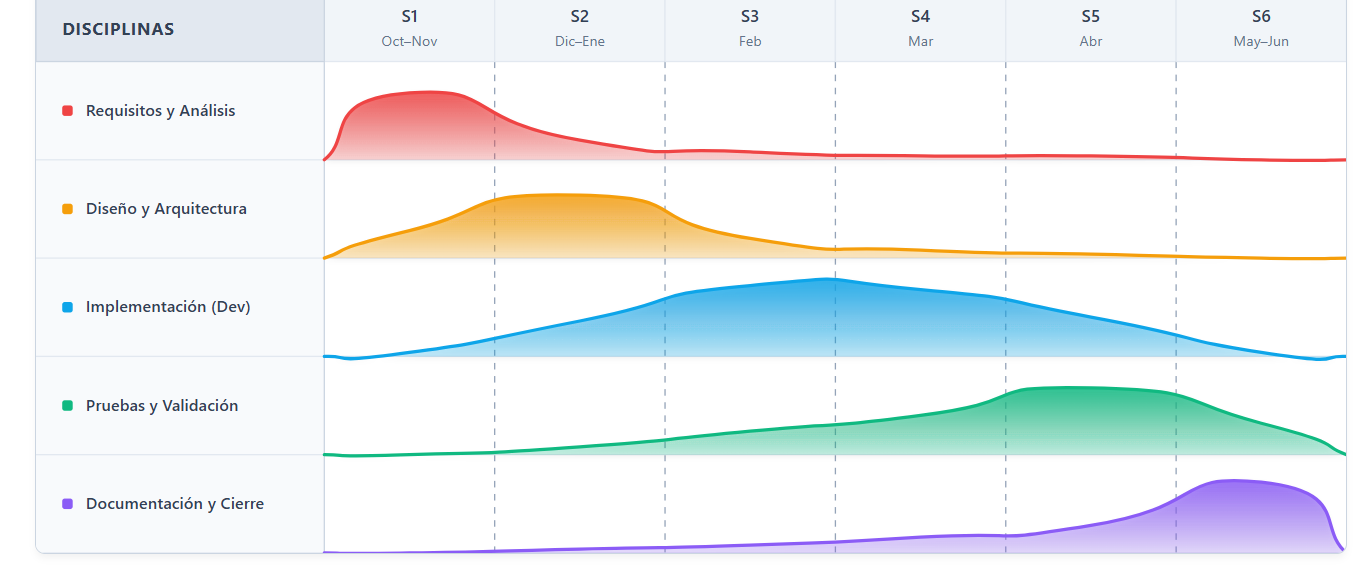
\includegraphics[width=1.2\textwidth]{figures/roadmap}%
  }
  \caption{Roadmap del proyecto: hitos entregados por sprint}
  \label{fig:roadmap}
\end{figure}

\begin{figure}[htbp]
  \centering
  \makebox[\textwidth][c]{%
    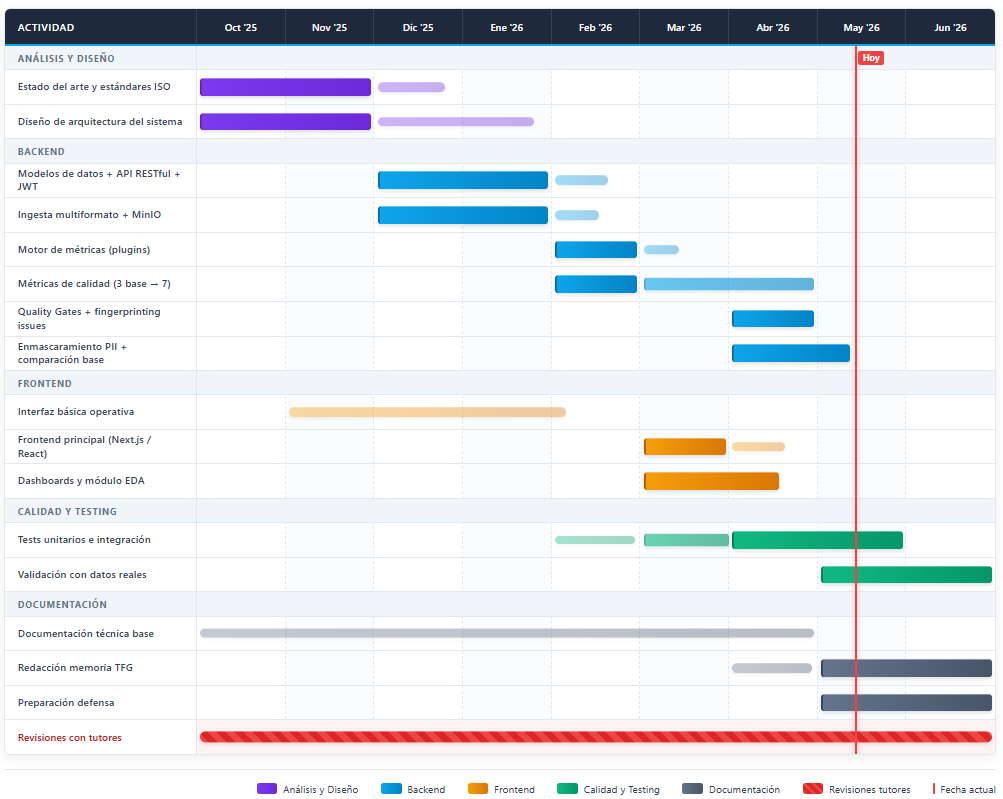
\includegraphics[width=1.2\textwidth]{figures/gantt}%
  }
  \caption{Diagrama de Gantt del proyecto (curso académico 2025--2026)}
  \label{fig:gantt}
\end{figure}

El diagrama de Gantt refleja el \emph{cuándo} de cada sprint, pero no la
intensidad relativa del trabajo en cada área.  La
Figura~\ref{fig:effort} muestra esa distribución de esfuerzo por disciplinas
y revela un patrón característico de los procesos ágiles: las actividades no
se suceden en fases estancas, sino que se solapan a lo largo del proyecto.

Los requisitos se concentran en el sprint inicial pero permanecen activos
durante todo el desarrollo.  El diseño y la arquitectura dominan los dos
primeros sprints y decaen progresivamente.  La implementación alcanza su pico
en los sprints centrales, mientras las pruebas crecen de forma sostenida a
medida que el sistema gana complejidad.  La documentación, presente desde el
inicio con un nivel de base, experimenta un salto significativo en el sprint
final.  Este patrón contrasta con la distribución secuencial del modelo en
cascada~\citep{sommerville2016}.

\begin{figure}[htbp]
  \centering
  \makebox[\textwidth][c]{%
    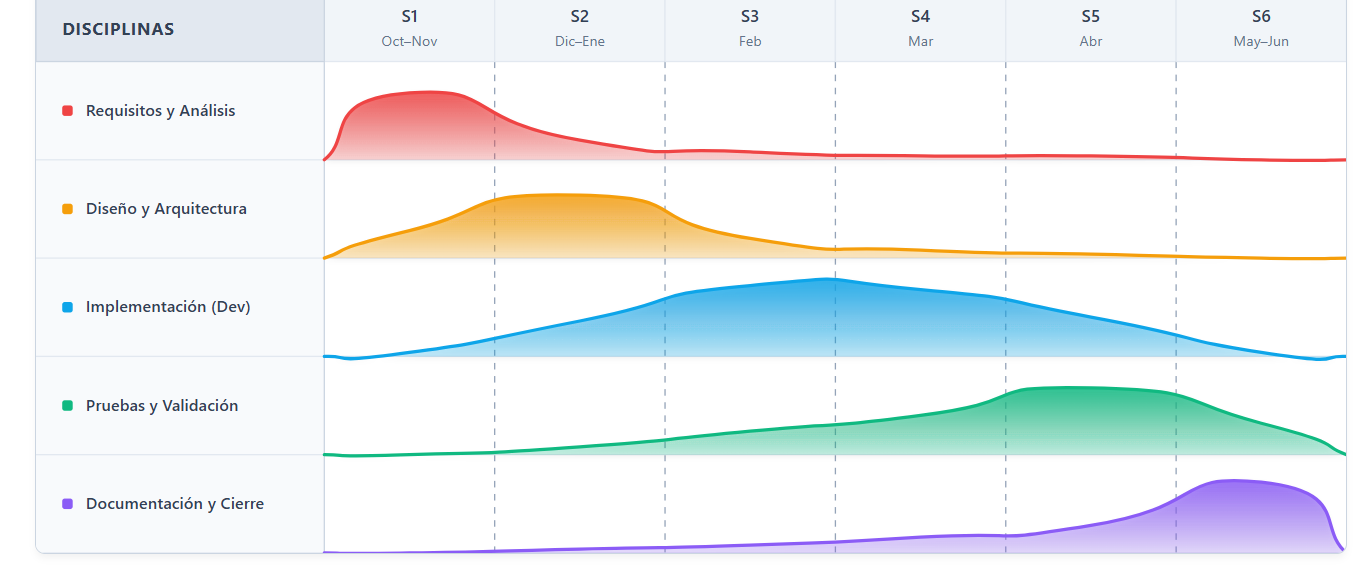
\includegraphics[width=1.2\textwidth]{figures/effort}%
  }
  \caption{Distribución de esfuerzo por disciplinas a lo largo de los sprints}
  \label{fig:effort}
\end{figure}


%% =========================================================================
\section{Backlog inicial e historias de usuario}
\label{sec:backlog-inicial}
%% =========================================================================

La Tabla~\ref{tab:backlog-hu} recoge el backlog inicial del proyecto,
organizado por épicas.  Cada historia de usuario sigue el formato
\textit{«Como [rol], quiero [acción] para [beneficio]»} y se estima en
\emph{story points} (SP) usando la escala de Fibonacci.  El backlog completo
con la asignación a sprints se incluye en el Anexo~C.

\begin{table}[htbp]
  \centering
  \small
  \caption{Backlog inicial — historias de usuario principales}
  \label{tab:backlog-hu}
  \begin{tabularx}{\textwidth}{l l X c c}
    \toprule
    \textbf{ID} & \textbf{Épica} & \textbf{Historia de usuario} &
      \textbf{Prior.} & \textbf{SP} \\
    \midrule
    HU-01 & Auth    & Como usuario, quiero registrarme con email y contraseña
      para acceder a la plataforma. & Alta & 3 \\
    HU-02 & Auth    & Como usuario, quiero iniciar sesión y recibir un JWT para
      autenticar mis peticiones. & Alta & 2 \\
    HU-03 & Proyectos & Como usuario, quiero crear un proyecto para agrupar
      conjuntos de datos relacionados. & Alta & 3 \\
    HU-04 & Proyectos & Como usuario, quiero ver el resumen de calidad de mi
      proyecto en un cuadro de mando. & Alta & 5 \\
    HU-05 & Datasets  & Como usuario, quiero cargar un fichero CSV
      para evaluarlo. & Alta & 5 \\
    HU-06 & Datasets  & Como usuario, quiero ver el versionado de mis datasets
      para rastrear cambios. & Media & 3 \\
    HU-07 & Métricas  & Como usuario, quiero configurar métricas con umbrales
      personalizados para adaptar la evaluación. & Alta & 5 \\
    HU-08 & Métricas  & Como usuario, quiero usar plantillas de métricas para
      reutilizar configuraciones. & Media & 3 \\
    HU-09 & Evaluación & Como usuario, quiero lanzar una evaluación y ver el
      progreso en tiempo real. & Alta & 8 \\
    HU-10 & Evaluación & Como usuario, quiero ver los problemas detectados con
      su severidad y columna afectada. & Alta & 5 \\
    HU-11 & Quality Gates & Como usuario, quiero definir un Quality Gate para
      saber si mi dataset es apto. & Alta & 5 \\
    HU-12 & Fingerprinting & Como usuario, quiero que los issues se tracen
      entre evaluaciones para detectar recurrencias. & Media & 8 \\
    HU-13 & EDA       & Como usuario, quiero explorar distribuciones, nulos y
      correlaciones de mis datos visualmente. & Media & 8 \\
    HU-14 & PII       & Como usuario, quiero marcar columnas sensibles para que
      sus valores no aparezcan en resultados. & Media & 5 \\
    HU-15 & Admin     & Como administrador, quiero gestionar usuarios y ver el
      estado del sistema. & Baja & 3 \\
    \midrule
    \multicolumn{4}{r}{\textbf{Total SP}} & \textbf{71} \\
    \bottomrule
  \end{tabularx}
\end{table}

El backlog inicial suma \textbf{71 puntos de historia}, distribuidos
principalmente en las épicas de mayor valor funcional: Evaluación,
\emph{Fingerprinting} y \ac{EDA}.  Las historias de prioridad baja
(HU-15) se planificaron para los últimos sprints y se implementaron
condicionadas a la disponibilidad de tiempo tras completar el núcleo
del sistema.


%% =========================================================================
\section{Estimación de esfuerzo}
\label{sec:estimacion}
%% =========================================================================

\subsection{Técnica de estimación}

La estimación del esfuerzo combinó dos técnicas complementarias con
distinto nivel de granularidad.  A nivel de historia de usuario se
emplearon \emph{story points} para capturar la complejidad relativa
sin comprometerse con una duración absoluta; a nivel de tarea técnica
se estimó directamente en horas para facilitar el seguimiento diario
en Trello.

\begin{itemize}
  \item \textbf{\emph{Story Points} con escala de Fibonacci} para la
    estimación relativa de las historias de usuario (véase
    Tabla~\ref{tab:backlog-hu}).  Se estableció una equivalencia
    orientativa de 4~horas por punto, lo que arroja una estimación
    base de 284~horas para las 71~SP del backlog.

  \item \textbf{Descomposición en tareas y estimación en horas} para
    las tareas técnicas más granulares registradas en Trello, así como
    para el sprint de documentación (S6), que no tiene historias de
    usuario asociadas y se estimó íntegramente en horas.
\end{itemize}

La Tabla~\ref{tab:estimacion-sprints} recoge la comparación entre la
estimación inicial y el tiempo real invertido en cada sprint.

\subsection{Estimación inicial vs.\ real}

\begin{table}[htbp]
  \centering
  \caption{Estimación inicial vs.\ real por sprint}
  \label{tab:estimacion-sprints}
  \begin{tabularx}{\textwidth}{l X c c c}
    \toprule
    \textbf{Sprint} & \textbf{Objetivo} &
      \textbf{SP} & \textbf{Est. (h)} & \textbf{Real (h)} \\
    \midrule
    S1 & Análisis, arquitectura y setup inicial  & 13 &  52 &  60 \\
    S2 & Backend core (auth, datasets, API REST) & 18 &  72 &  85 \\
    S3 & Motor de métricas (7 métricas)          & 16 &  64 &  70 \\
    S4 & Frontend y visualizaciones              & 14 &  56 &  65 \\
    S5 & Features avanzadas (fingerprinting, QG, PII) & 10 & 40 & 55 \\
    S6 & Documentación, pruebas y defensa        &  0 &  80 &  90 \\
    \midrule
    \textbf{Total} & & \textbf{71} & \textbf{364} & \textbf{425} \\
    \bottomrule
  \end{tabularx}
\end{table}

La desviación media del \textbf{+16,8\,\%} sobre la estimación inicial es
consistente con la literatura sobre proyectos de software de tamaño similar,
y se explica principalmente por la subestimación del tiempo de configuración
de la infraestructura Docker (S1), la complejidad del parseo robusto de CSV
(S2) y la implementación del sistema de fingerprinting (S5).


%% =========================================================================
\section{Estimación de costes}
\label{sec:costes}
%% =========================================================================

Con el objetivo de proporcionar una perspectiva de viabilidad económica,
se estima el coste que tendría el proyecto en un entorno profesional real.

\begin{table}[htbp]
  \centering
  \caption{Estimación de costes del proyecto}
  \label{tab:costes}
  \begin{tabularx}{\textwidth}{l X c c c}
    \toprule
    \textbf{Concepto} & \textbf{Detalle} &
      \textbf{Cantidad} & \textbf{Precio unit.} & \textbf{Total} \\
    \midrule
    \multicolumn{5}{l}{\textit{Recursos humanos}} \\
    Desarrollador \emph{full-stack} (junior) &
      425 h de desarrollo real & 425~h & 25~€/h & 10\,625~€ \\
    \midrule
    \multicolumn{5}{l}{\textit{Licencias de software}} \\
    Python, Flask, Next.js, PostgreSQL\ldots &
      Todo el stack es \emph{open source} & --- & 0~€ & 0~€ \\
    GitHub (plan Free)                       &
      Repositorio de código y control de versiones  &  1  & 0~€ & 0~€ \\
    \midrule
    \multicolumn{5}{l}{\textit{Infraestructura}} \\
    Hardware de desarrollo &
      Amortización del equipo propio (1\,000~€ / 36 meses $\times$ 9 meses)
      & 1 & 250~€ & 250~€ \\
    Servicios cloud        &
      Despliegue local con Docker Compose    & --- & 0~€ & 0~€ \\
    \midrule
    \multicolumn{4}{r}{\textbf{Coste total estimado}} & \textbf{10\,875~€} \\
    \bottomrule
  \end{tabularx}
\end{table}

El coste total estimado de \textbf{10\,875~€} se desglosa en 10\,625~€ de
mano de obra a tarifa de desarrollador junior y 250~€ de amortización del
equipo de desarrollo (portátil valorado en 1\,000~€, vida útil de 3~años,
uso durante 9~meses).  Dado que todas las tecnologías utilizadas son de
código abierto y el despliegue es local, el coste de licencias es nulo.  Para un escenario de
producción con despliegue en nube (AWS, Azure), debería añadirse el coste de
los servicios equivalentes (RDS, S3, ElastiCache, ECS), estimado en
unos 150--300~€/mes según el volumen de uso.


%% =========================================================================
\section{Gestión de riesgos}
\label{sec:riesgos}
%% =========================================================================

La gestión de riesgos se realizó de forma proactiva al inicio del
proyecto, identificando los principales factores de riesgo y definiendo
acciones preventivas y correctivas para cada uno.  El seguimiento se
llevó a cabo en las retrospectivas de cada sprint, donde se evaluaba si
algún riesgo se había materializado y si las acciones aplicadas habían
sido efectivas.

La Tabla~\ref{tab:riesgos} recoge los riesgos identificados con su
probabilidad de ocurrencia (Alta/Media/Baja), impacto (Alto/Medio/Bajo)
y las acciones definidas.

\begin{table}[htbp]
  \centering
  \small
  \caption{Plan de gestión de riesgos}
  \label{tab:riesgos}
  \begin{tabularx}{\textwidth}{l >{\raggedright\arraybackslash}X c c >{\raggedright\arraybackslash}X >{\raggedright\arraybackslash}X}
    \toprule
    \textbf{ID} & \textbf{Riesgo} & \textbf{Prob.} & \textbf{Imp.} &
      \textbf{Acción preventiva} & \textbf{Acción correctiva} \\
    \midrule
    R-01 & Complejidad mayor de lo esperada en el motor de métricas
      & Media & Alto
      & Reservar un sprint completo (S3) para esta fase
      & Reducir el número de métricas en el MVP inicial \\
    R-02 & Problemas de integración entre servicios Docker
      & Media & Alto
      & Levantar el stack completo desde el sprint~1
      & Acotar el \emph{healthcheck} y consultar documentación oficial \\
    R-03 & Desvío temporal por subestimación de tareas
      & Alta  & Medio
      & Añadir un 20\,\% de margen en cada sprint
      & Repriorizar el backlog y mover HU a sprints siguientes \\
    R-04 & Pérdida de datos o código por accidente
      & Baja  & Alto
      & Repositorio en GitHub con \emph{push} frecuente
      & Restaurar desde el último \emph{commit} \\
    R-05 & Cambios de requisitos por retroalimentación de tutores
      & Media & Medio
      & Revisiones bajo demanda con los tutores para detectar desviaciones
      & Incorporar cambios al backlog en la siguiente sprint planning \\
    R-06 & Problemas de rendimiento con ficheros grandes
      & Media & Medio
      & Establecer límite de 100\,MB configurado en el servidor
      & Añadir endpoint de estado y aviso al usuario \\
    R-07 & Fallos en la autenticación JWT en producción
      & Baja  & Alto
      & Pruebas de integración del flujo auth completo
      & Revisión de configuración de expiración y \emph{blacklisting} \\
    R-08 & Incompatibilidad de versiones entre dependencias
      & Media & Medio
      & Fijar versiones en \texttt{requirements.txt} y \texttt{package.json}
      & Revertir a la versión compatible e investigar la causa \\
    \bottomrule
  \end{tabularx}
\end{table}

De los ocho riesgos identificados, tres se materializaron durante el
desarrollo: R-03 (desvío temporal) en los sprints S2 y S5, R-02
(integración Docker) en S5 con el sistema Celery+Redis, y R-08
(incompatibilidad de versiones) durante la migración de SQLAlchemy
1.x a 2.0 en S2.  Los cinco riesgos restantes no llegaron a
producirse, lo que valida en parte las acciones preventivas adoptadas.
El análisis detallado de ocurrencia se recoge en el Anexo~D.


% Local Variables:
%  coding: utf-8
%  mode: latex
%  mode: flyspell
%  ispell-local-dictionary: "castellano8"
% End:
